\documentclass[a4paper]{article}
\usepackage{amsmath}
%\usepackage{graphicx}

\title{The Error Function}
\author{Guillermo Garrido Hernández}

\begin{document}
\maketitle

\begin{abstract}
In mathematics, the error function (also called the Gauss error function) is a
special function (non-elementary) of sigmoid shape that occurs in probability,
statistics, and partial differential equations describing diffusion.
It is defined as:
$erf(x) = \frac{2}{\sqrt{\pi}}\int_0^\infty e^{-t^2}dt$.
In statistics, for nonnegative values of x, the error function has the following
interpretation: for a random variable Y that is normally distributed with mean 0
and variance 1/2, erf(x) describes the probability of Y falling in the range
[-x, x].
\end{abstract}

\section{Name}
The name and abbreviation for the error function (and the error function
complement) were developed by J. W. L. Glaisher in 1871 on account of its
connection with "the theory of Probability, and notably the theory of Errors."

\section{Properties}
The property $erf(-z)=−erf(z)$  means that the
error function is an odd function. This directly results from the fact that the
integrand $e^{-t^2}$ is an even function.

For any complex number $z$:
\begin{equation}
  erf(\bar{z})=\bar{erf(z)}
\end{equation}
where $\bar{z}$ is the complex conjugate of $z$.

The error function at $+\infty$ is exactly $1$ (see Gaussian integral). At the
real axis, $erf(z)$ approaches unity at $z\rightarrow\infty$ and
$-1$ at $z\rightarrow -\infty$. At the imaginary axis, it tends to $\pm i\infty$.

The error function is an entire function; it has no singularities (except that at
infinity) and its Taylor expansion always converges.

The shape of the error function can be seen in Figure \ref{fig}.
\begin{figure}
  % GNUPLOT: LaTeX picture
\setlength{\unitlength}{0.240900pt}
\ifx\plotpoint\undefined\newsavebox{\plotpoint}\fi
\sbox{\plotpoint}{\rule[-0.200pt]{0.400pt}{0.400pt}}%
\begin{picture}(1500,900)(0,0)
\sbox{\plotpoint}{\rule[-0.200pt]{0.400pt}{0.400pt}}%
\put(171.0,131.0){\rule[-0.200pt]{4.818pt}{0.400pt}}
\put(151,131){\makebox(0,0)[r]{$-1$}}
\put(1419.0,131.0){\rule[-0.200pt]{4.818pt}{0.400pt}}
\put(171.0,204.0){\rule[-0.200pt]{4.818pt}{0.400pt}}
\put(151,204){\makebox(0,0)[r]{$-0.8$}}
\put(1419.0,204.0){\rule[-0.200pt]{4.818pt}{0.400pt}}
\put(171.0,276.0){\rule[-0.200pt]{4.818pt}{0.400pt}}
\put(151,276){\makebox(0,0)[r]{$-0.6$}}
\put(1419.0,276.0){\rule[-0.200pt]{4.818pt}{0.400pt}}
\put(171.0,349.0){\rule[-0.200pt]{4.818pt}{0.400pt}}
\put(151,349){\makebox(0,0)[r]{$-0.4$}}
\put(1419.0,349.0){\rule[-0.200pt]{4.818pt}{0.400pt}}
\put(171.0,422.0){\rule[-0.200pt]{4.818pt}{0.400pt}}
\put(151,422){\makebox(0,0)[r]{$-0.2$}}
\put(1419.0,422.0){\rule[-0.200pt]{4.818pt}{0.400pt}}
\put(171.0,495.0){\rule[-0.200pt]{4.818pt}{0.400pt}}
\put(151,495){\makebox(0,0)[r]{$0$}}
\put(1419.0,495.0){\rule[-0.200pt]{4.818pt}{0.400pt}}
\put(171.0,567.0){\rule[-0.200pt]{4.818pt}{0.400pt}}
\put(151,567){\makebox(0,0)[r]{$0.2$}}
\put(1419.0,567.0){\rule[-0.200pt]{4.818pt}{0.400pt}}
\put(171.0,640.0){\rule[-0.200pt]{4.818pt}{0.400pt}}
\put(151,640){\makebox(0,0)[r]{$0.4$}}
\put(1419.0,640.0){\rule[-0.200pt]{4.818pt}{0.400pt}}
\put(171.0,713.0){\rule[-0.200pt]{4.818pt}{0.400pt}}
\put(151,713){\makebox(0,0)[r]{$0.6$}}
\put(1419.0,713.0){\rule[-0.200pt]{4.818pt}{0.400pt}}
\put(171.0,785.0){\rule[-0.200pt]{4.818pt}{0.400pt}}
\put(151,785){\makebox(0,0)[r]{$0.8$}}
\put(1419.0,785.0){\rule[-0.200pt]{4.818pt}{0.400pt}}
\put(171.0,858.0){\rule[-0.200pt]{4.818pt}{0.400pt}}
\put(151,858){\makebox(0,0)[r]{$1$}}
\put(1419.0,858.0){\rule[-0.200pt]{4.818pt}{0.400pt}}
\put(171.0,131.0){\rule[-0.200pt]{0.400pt}{4.818pt}}
\put(171,90){\makebox(0,0){$-3$}}
\put(171.0,838.0){\rule[-0.200pt]{0.400pt}{4.818pt}}
\put(382.0,131.0){\rule[-0.200pt]{0.400pt}{4.818pt}}
\put(382,90){\makebox(0,0){$-2$}}
\put(382.0,838.0){\rule[-0.200pt]{0.400pt}{4.818pt}}
\put(594.0,131.0){\rule[-0.200pt]{0.400pt}{4.818pt}}
\put(594,90){\makebox(0,0){$-1$}}
\put(594.0,838.0){\rule[-0.200pt]{0.400pt}{4.818pt}}
\put(805.0,131.0){\rule[-0.200pt]{0.400pt}{4.818pt}}
\put(805,90){\makebox(0,0){$0$}}
\put(805.0,838.0){\rule[-0.200pt]{0.400pt}{4.818pt}}
\put(1016.0,131.0){\rule[-0.200pt]{0.400pt}{4.818pt}}
\put(1016,90){\makebox(0,0){$1$}}
\put(1016.0,838.0){\rule[-0.200pt]{0.400pt}{4.818pt}}
\put(1228.0,131.0){\rule[-0.200pt]{0.400pt}{4.818pt}}
\put(1228,90){\makebox(0,0){$2$}}
\put(1228.0,838.0){\rule[-0.200pt]{0.400pt}{4.818pt}}
\put(1439.0,131.0){\rule[-0.200pt]{0.400pt}{4.818pt}}
\put(1439,90){\makebox(0,0){$3$}}
\put(1439.0,838.0){\rule[-0.200pt]{0.400pt}{4.818pt}}
\put(171.0,131.0){\rule[-0.200pt]{0.400pt}{175.134pt}}
\put(171.0,131.0){\rule[-0.200pt]{305.461pt}{0.400pt}}
\put(1439.0,131.0){\rule[-0.200pt]{0.400pt}{175.134pt}}
\put(171.0,858.0){\rule[-0.200pt]{305.461pt}{0.400pt}}
\put(30,494){\makebox(0,0){$y$}}
\put(805,29){\makebox(0,0){$x$}}
\put(1279,817){\makebox(0,0)[r]{erf$(x)$}}
\put(1299.0,817.0){\rule[-0.200pt]{24.090pt}{0.400pt}}
\put(171,131){\usebox{\plotpoint}}
\put(298,130.67){\rule{10.118pt}{0.400pt}}
\multiput(298.00,130.17)(21.000,1.000){2}{\rule{5.059pt}{0.400pt}}
\put(340,131.67){\rule{10.118pt}{0.400pt}}
\multiput(340.00,131.17)(21.000,1.000){2}{\rule{5.059pt}{0.400pt}}
\put(382,133.17){\rule{8.700pt}{0.400pt}}
\multiput(382.00,132.17)(24.943,2.000){2}{\rule{4.350pt}{0.400pt}}
\multiput(425.00,135.59)(4.606,0.477){7}{\rule{3.460pt}{0.115pt}}
\multiput(425.00,134.17)(34.819,5.000){2}{\rule{1.730pt}{0.400pt}}
\multiput(467.00,140.59)(2.739,0.488){13}{\rule{2.200pt}{0.117pt}}
\multiput(467.00,139.17)(37.434,8.000){2}{\rule{1.100pt}{0.400pt}}
\multiput(509.00,148.58)(1.330,0.494){29}{\rule{1.150pt}{0.119pt}}
\multiput(509.00,147.17)(39.613,16.000){2}{\rule{0.575pt}{0.400pt}}
\multiput(551.00,164.58)(0.900,0.496){45}{\rule{0.817pt}{0.120pt}}
\multiput(551.00,163.17)(41.305,24.000){2}{\rule{0.408pt}{0.400pt}}
\multiput(594.00,188.58)(0.567,0.498){71}{\rule{0.554pt}{0.120pt}}
\multiput(594.00,187.17)(40.850,37.000){2}{\rule{0.277pt}{0.400pt}}
\multiput(636.58,225.00)(0.498,0.595){81}{\rule{0.120pt}{0.576pt}}
\multiput(635.17,225.00)(42.000,48.804){2}{\rule{0.400pt}{0.288pt}}
\multiput(678.58,275.00)(0.498,0.763){81}{\rule{0.120pt}{0.710pt}}
\multiput(677.17,275.00)(42.000,62.527){2}{\rule{0.400pt}{0.355pt}}
\multiput(720.58,339.00)(0.498,0.874){83}{\rule{0.120pt}{0.798pt}}
\multiput(719.17,339.00)(43.000,73.344){2}{\rule{0.400pt}{0.399pt}}
\multiput(763.58,414.00)(0.498,0.967){81}{\rule{0.120pt}{0.871pt}}
\multiput(762.17,414.00)(42.000,79.191){2}{\rule{0.400pt}{0.436pt}}
\multiput(805.58,495.00)(0.498,0.955){81}{\rule{0.120pt}{0.862pt}}
\multiput(804.17,495.00)(42.000,78.211){2}{\rule{0.400pt}{0.431pt}}
\multiput(847.58,575.00)(0.498,0.874){83}{\rule{0.120pt}{0.798pt}}
\multiput(846.17,575.00)(43.000,73.344){2}{\rule{0.400pt}{0.399pt}}
\multiput(890.58,650.00)(0.498,0.763){81}{\rule{0.120pt}{0.710pt}}
\multiput(889.17,650.00)(42.000,62.527){2}{\rule{0.400pt}{0.355pt}}
\multiput(932.58,714.00)(0.498,0.595){81}{\rule{0.120pt}{0.576pt}}
\multiput(931.17,714.00)(42.000,48.804){2}{\rule{0.400pt}{0.288pt}}
\multiput(974.00,764.58)(0.567,0.498){71}{\rule{0.554pt}{0.120pt}}
\multiput(974.00,763.17)(40.850,37.000){2}{\rule{0.277pt}{0.400pt}}
\multiput(1016.00,801.58)(0.900,0.496){45}{\rule{0.817pt}{0.120pt}}
\multiput(1016.00,800.17)(41.305,24.000){2}{\rule{0.408pt}{0.400pt}}
\multiput(1059.00,825.58)(1.330,0.494){29}{\rule{1.150pt}{0.119pt}}
\multiput(1059.00,824.17)(39.613,16.000){2}{\rule{0.575pt}{0.400pt}}
\multiput(1101.00,841.59)(2.739,0.488){13}{\rule{2.200pt}{0.117pt}}
\multiput(1101.00,840.17)(37.434,8.000){2}{\rule{1.100pt}{0.400pt}}
\multiput(1143.00,849.59)(4.606,0.477){7}{\rule{3.460pt}{0.115pt}}
\multiput(1143.00,848.17)(34.819,5.000){2}{\rule{1.730pt}{0.400pt}}
\put(1185,854.17){\rule{8.700pt}{0.400pt}}
\multiput(1185.00,853.17)(24.943,2.000){2}{\rule{4.350pt}{0.400pt}}
\put(1228,855.67){\rule{10.118pt}{0.400pt}}
\multiput(1228.00,855.17)(21.000,1.000){2}{\rule{5.059pt}{0.400pt}}
\put(1270,856.67){\rule{10.118pt}{0.400pt}}
\multiput(1270.00,856.17)(21.000,1.000){2}{\rule{5.059pt}{0.400pt}}
\put(171.0,131.0){\rule[-0.200pt]{30.594pt}{0.400pt}}
\put(1312.0,858.0){\rule[-0.200pt]{20.476pt}{0.400pt}}
\put(171.0,131.0){\rule[-0.200pt]{0.400pt}{175.134pt}}
\put(171.0,131.0){\rule[-0.200pt]{305.461pt}{0.400pt}}
\put(1439.0,131.0){\rule[-0.200pt]{0.400pt}{175.134pt}}
\put(171.0,858.0){\rule[-0.200pt]{305.461pt}{0.400pt}}
\end{picture}

  %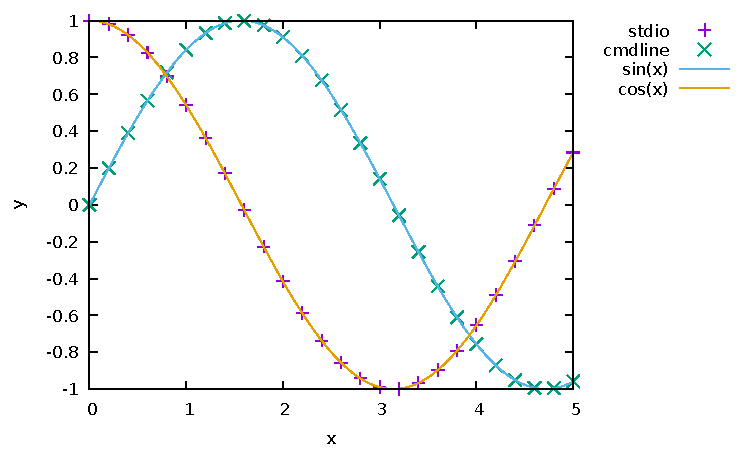
\includegraphics[scale=0.9]{plot.jpg}
  \caption{A plot of the error function calculated from the differential equation.}
  \label{fig}
\end{figure}
\end{document}
